%%%%%%%%%%%%%%%%%%%%%%%%%%%%%%%%%%%%%%%%%%%%%%%%%%%%%%%%%%%%%%%%%%%%%%%%%%%%%%%
\section{Aberration Measurement and Correction}
\label{Measurement}
%%%%%%%%%%%%%%%%%%%%%%%%%%%%%%%%%%%%%%%%%%%%%%%%%%%%%%%%%%%%%%%%%%%%%%%%%%%%%%%

In practice, no optical system can be totally free from aberrations. That means that all the rays coming from the same object point and going through an optical system will not converge into the same point at the image plane. In other words, the wavefront is distorted with respect an ideal one when passing through a real system. Thus, we can define the Wavefront Aberration Function as the optical path difference between the aberrated (real) wavefront and the reference (perfect) wavefront.      
There are some ways to characterize mathematically the aberrations. In systems with circular symmetry (circular apertures) it is very common to use the Zernike polynomials \eqref{eq:aberration_zernike}  because they form a complete, orthogonal set of functions defined over a unit circle. This property gives independence between these functions. That implies that it is possible to associate to each polynomial a specific an independent weight that will contribute to the description of the Wavefront Aberration Function.  

\begin{align}
	\ W(\rho,\phi) = {\sum_{n}^{k}}{\sum_{m=-n}^{m=n}}{{c_n}^m {Z_n}^m}{(\rho,\phi)},
	\label{eq:aberration_zernike}
\end{align}

Where $W(\rho,\phi)$ is the Wavefront Aberration Function in polar coordinates at the exit pupil, $c_n^m$ are the Zernike coefficients and $Z_n^m (\rho,\phi)$ are the Zernike modes (or polynomials). As we can see in the equation, the Wavefront Aberration Function is a linear combination of polynomials. Therefore, the more polynomials (i.e. modes, $Z_n^m (\rho,\phi)$) we get the better characterization of the $W(\rho,\phi)$ function we have.
Representing aberrations in this way can simplify the design, control and characterization of the Adaptive Optics system. 
In general, we can obtain an aberrated wavefront when it is reflected to a non-planar surface or when it is going through an inhomogeneous media (Fig. \ref{fig:abberations}). 

\begin{figure}[tbh]
       \centering
        \begin{subfigure}[b]{0.4\textwidth}
                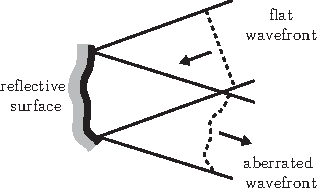
\includegraphics[width=\textwidth]{images/wavefront_distortions_reflection}
                \caption{Reflection.}
                \label{fig:abberation_reflection}
        \end{subfigure}
				\hspace{1em}
        \begin{subfigure}[b]{0.3\textwidth}
                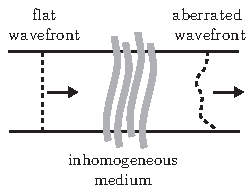
\includegraphics[width=\textwidth]{images/wavefront_distortions_transmission}
                \caption{Transmission.}
                \label{fig:abberation_trans}
        \end{subfigure}
        \caption{Wavefront aberrations due to (a) reflection from a non 
planar surface and (b)  caused by propagation through a non-uniform 
refractive index distribution \cite{AOM_basic_ref}.}
\label{fig:abberations}
\end{figure} 

In biological microscopy, the two potential sources of aberrations are the optics and the specimen under study. Regarding the optics, one important parameter that has to be taken into account is the Numerical Aperture (NA), aberrations become more significant for those microscopes employing higher NA. Regarding the specimen, aberrations comes basically from the variations in refractive index due to the three-dimensional nature of cells and tissue structures. In general, they become greater in magnitude as long as we focus deeper. Also aberrations can be produced by the difference of refractive index between the microscope coverslip and the specimen mounting medium \cite{AOM_basic_ref}. 
Although it is known where the aberrations come from, it is not always easy to measure them and implement the measure inside the optical system. There are different classifications of Wavefront Sensing in the bibliography \cite{AO_engineering_handbook}. Here we will use the one of Martin J. Booth \cite{AOM_basic_ref} and we will explain the most common methods of wavefront sensing applied to microscopy.      


%%%%%%%%%%%%%%%%%%%%%%%%%%%%%%%%%%%%%%%%%%%%%%%%%%%%%%%%%%%%%%%%%%%%%%%%%%%%%%%
\subsection{Direct Wavefront Sensing}
\label{sec:WavefrontSensing}
Direct Wavefront Sensing is based on a direct measure of the phase gradient or the wavefront slope, it is considered as an aperture-plane sensing. Within this group there are several techniques such as interferometric, although in general the most used is the Shack-Hartmann. 

%------------------------------------------------------------------------------

This last technique has its origin more than 400 years ago in the Scheiner's Disk developed by the astronomer Christopher Scheiner \cite{Principles_HS}. Later on, in the twenty century, Hartmann used the Scheiner's Disk to develop a test which measured the wavefront's slope at the exit of the optical system by using a screen with multiple holes. This technique was progressing until the 1971, when Platt and Shack developed a two-dimensional array of a few lenslets -a matrix of microlens-, all with the same diameter and the same focal length, that could substitute the screen with multiple holes. This is the start point of the technique known as "`Shack-Hartmann"'\cite{History_HS}.
  
This technique allows us to reconstruct the wavefront aberration function from the local slope's changes of an aberrated wavefront in relation with a reference wavefront. That is achieved measuring the displacements ($\Delta x, \Delta y$) from each image given by each microlent (Fig. \ref{fig:SH}).

\begin{figure}[htbp]
	\centering
		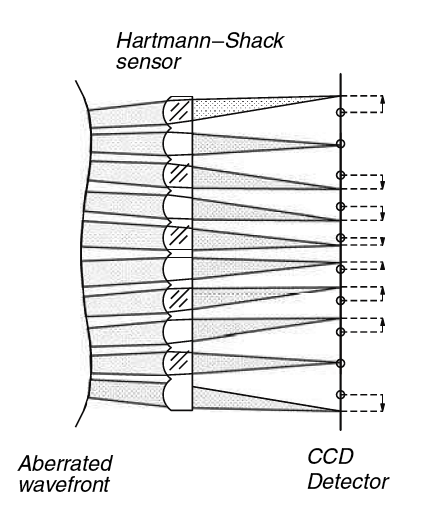
\includegraphics[width=0.35\textwidth]{images/SH.png}
	\caption{Two-dimensional section of Shack-Hartmann matrix of microlens. When an incoming wavefront goes through the matrix is divided in multiple beams. In the focal plane of the matrix we have multiple spots. If the wavefront is not aberrated each spot will be placed in the axis of each microlens. If it is aberrated, it will be displaced with respect this axis \cite{optical_shop_testing}.}
	\label{fig:SH}
\end{figure}


We start from an aberrated beam going through the matrix of microlens before it is detected in a recorder device. The beam is then spatially sampled into many individual beams (one for each microlens) by the lenslet matrix and forms multiple spots in the focal plane of the lenslets. Finally, the recorder device -that is placed at the focal plane of the matrix- registers multiple spots. This device is usually a CCD camera. The typical lenslet diameters range from about 100 to 600 mm and the typical focal lengths range from a few millimeters to about 30 mm \cite{AO_vision_science}.
  
We must note that direct sensing needs a well defined wavefront in the pupil of the system or in other words, a point-like emitter. An this situation might not happen in biological microscopes where we are studying three-dimensional specimens, because the light emitted by the specimen may come not only from the focal point. This fact brings us to a couple of problematic situations. The first one is the superposition of wavefronts in the pupil which its effects will depend on the coherence of the emitted light. If it is coherent we will have interference in the pupil, thus we will have ambiguous sensor readings and this kind of sensing will not be suitable for aberration correction. In this sense, if in the focal region the specimen behaves as a point-like scatterer (it will emit incoherent light) the sensor will be able to measure the aberrations produced in the emission path, which in principle they should be the same as in the illumination path. But, if our specimen acts as a planar mirror-like in the focal region, the sensor will just be able to measure twice the even components of the aberrations produced in the illumination path (or emission path), that is because the "`mirror behaviour"' will spatially invert the aberrations in the illumination path (Fig. \ref{fig:abe_direct_sensing}). 

\begin{figure}[htbp]
	\centering
		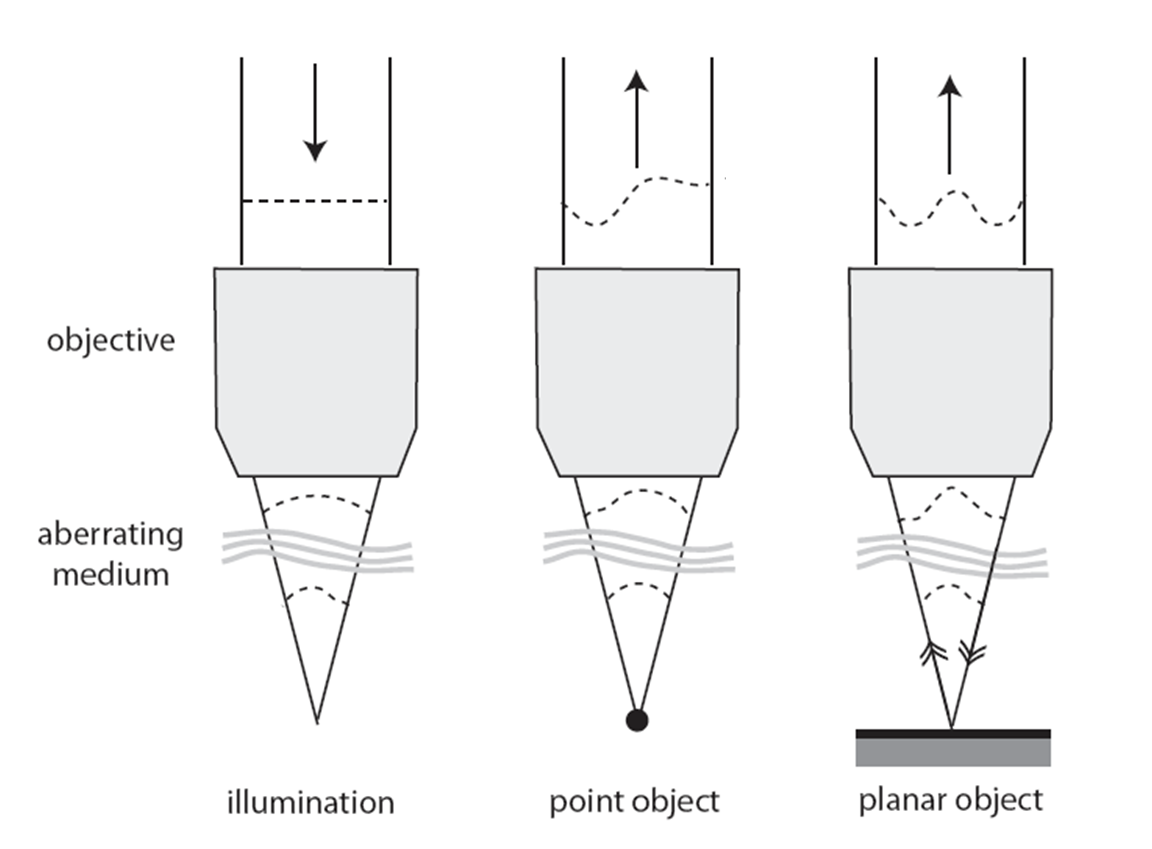
\includegraphics[width=0.45\textwidth]{images/abe_direct_sensing.png}
	\caption{Representation of the two effects due to the specimen structure on wavefront measurements. The left figure shows how the wavefront is aberrated in the illumination path. In the center it is shown a point-like scatterer. Only the emission path is measured. In the right figure it is shown a planar reflector. The illumination wavefront is spatially inverted on reflection before aquiring further aberration in the detection path \cite{AOM_basic_ref}.}
	\label{fig:abe_direct_sensing}
\end{figure}


Let us analyse it in detail. We denote the illumination ($W(\rho,\phi)_i)$ and emission ($W(\rho,\phi)_e$) path aberrations as the sum of its even and odd components,

\begin{align}
	\ W(\rho,\phi)_i = {{W(\rho,\phi)_i}^{even}} + {{W(\rho,\phi)_i}^{odd}},
	\label{eq:aberration_i_even_odd_sum}
\end{align}   

\begin{align}
	\ W(\rho,\phi)_e = {{W(\rho,\phi)_e}^{even}} + {{W(\rho,\phi)_e}^{odd}},
	\label{eq:aberration_e_even_odd_sum}
\end{align}   

The measured aberration ($W(\rho,\phi)$) is the sum of the illumination and emission path aberrations,

\begin{align}
	\ W(\rho,\phi) = {{W(\rho,\phi)_i}^{even}} + {{W(\rho,\phi)_i}^{odd}}+{{W(\rho,\phi)_e}^{even}} + {{W(\rho,\phi)_e}^{odd}},
	\label{eq:aberration_sum_il_em}
\end{align}  

Due to the spatial inversion we know that,

\begin{align}
	\ W(\rho,\phi)_i^{even}={{W(\rho,\phi)_e}^{even}}
	\label{eq:spat_inversion_even}
\end{align}
	
\begin{align}
	\ W(\rho,\phi)_e^{odd}=-{{W(\rho,\phi)_e}^{odd}}
	\label{eq:spat_inversion_odd}
\end{align} 

Then, the aberration measured can be simplified, 

\begin{align}
	\ W(\rho,\phi)=2 {{W(\rho,\phi)_e}}
	\label{eq:ab_measured_spat_inver}
\end{align} 

We have shown that in planar mirror-like structures we lose information about aberrations. Thus, in this cases it is not a good option to implement a direct sensing. Regarding microscopy techniques, we must note here that fluorescence emission is an incoherent process, but the non-linear processes generate a coherent signal.

The other problematic situation that we can have in direct sensing due to three-dimensional nature of the specimen is that our sensor might detect more intensity signal from the light scattered out-of-focus than the scattered in the focal region. In order to overcome this problem it can be used a spatial filter between objective and sensor. This filter performs in a similar way than the pinhole used in confocal microscopy. Also it is possible to use coherence gating to exclude out-of-focus light instead of the spatial filter, although it is a more complex method. We must recall here that the light emitted in the non-linear processes is confined mostly in the focal region.

%------------------------------------------------------------------------------

%%%%%%%%%%%%%%%%%%%%%%%%%%%%%%%%%%%%%%%%%%%%%%%%%%%%%%%%%%%%%%%%%%%%%%%%%%%%%%%
\subsection{Indirect Wavefront Sensing}
\label{sec:IndirectWavefrontSensing}

While direct wavefront sensing techniques are widely applied in Astronomy, 
they are less common in microscopy techniques. This for several reasons. It 
is not as easy to create a guiding start like point source in a biological 
specimen. If there are not features in the specimen that occur there 
naturally and which resemble a point source, one has to be implemented 
manually which might alter the function of the specimen or might even be 
toxic to the sample. Modern microscopes are also highly complex and 
optimized, which makes it difficult to insert a relatively large wavefront 
sensor. For samples with weak signal strength, it is also desirable to 
collect as many photons as possible for the imaging process. Splitting the 
beam and using a part of the light emitted from the sample for direct 
wavefront sensing might hence decrease the signal strength too much.

Indirect techniques do not measure the wavefront directly but instead 
optimize the image quality. This leads to the retrieval of the aberration and 
the necessary corrections. Hence these techniques don't sense the wavefront 
but rather improve the image quality and through this correct for wavefront 
aberrations. Indirect methods are used more often in industrial and medical 
applications. They usually require very little additional hardware. Once the 
technique is optimized for a specific problem, indirect schemes are easier to 
implement in practice and are more prone to errors due to the lack of 
additional hardware~(a single deformable mirror might be sufficient to 
implement adaptive optics in an existing microscope).

Indirect techniques include phase diversity as well as optimization of an 
image quality metric. Phase diversity techniques use two or more images of an 
extended object to make an estimation of the distorting wavefront~\cite{
indirect_phase_retrieval_algorithm}. However, this technique still requires a 
beam splitter, a second detector and a deformable mirror which is a 
significant disadvantage over image quality metric optimization where only 
the normally recorded image and a deformable mirror is required. It is also 
necessary to record images with different focus positions and hence the each 
phase retrieval step takes many seconds. Therefore the entire process of 
optimizing the wavefront takes minutes, which is to slow for most biological 
imaging~\cite{indirect_AOM_phase_retrieval}. It is for these reasons that 
phase diversity techniques are less common in microscopy and will not be 
described further. The focus of this section is therefor a general 
description of image quality metric techniques. Their specific properties and 
how they are implemented in the different microscopy techniques is then 
described in Section~\ref{sec:ExperimentDiscussion}. 

%------------------------------------------------------------------------------
%Optimization of an Image Quality Metric

The optimization of an image quality metric is mainly a mathematical rahter then a techniquel problem. We will describe the basic principle but the derivation of the specifc metrics is beyond the scope of this paper. The interested reader will find more information on the mathematical background in reference~\cite{wide_parabolic_optimization,wide_sphere_packing,wide_Lukosz_Modes,wide_AOM_loew_freq}. 

For these techniques, the aberration correction is performed through an iterative optimization of an image quality metric based. The metric is usually based on spatial frequencies~\cite{wide_AOM_loew_freq} or image intensity~\cite{indirect_metric_intensity}. Such optimization is either implemented empirically or by using an appropriate mathematical model. In many practical systems aberrations can be accurately represented by a small number of modes of an orthogonal basis, such as Zernikepolynomials. A sequence of images is acquired, each with a different aberration applied and the correction aberration is estimated from the information in this images. This process is repeated until the image quality is considered acceptable. The number of measurements needed to obtain an acceptable image depends strongly upon the optimization algorithm and parameters used, the mathematical representation of the aberration, and the object structure. For the earliest and most generic algorithms the number of measurements per aberration mode increases quadratically or exponentially with $N$, the number of corrected aberration modes~\cite{wide_sphere_packing}. The so called direct maximization method~(as described in Section~\ref{sec:TransmissionMicroscope}) is significantly more efficient, requiring only $N+1$ measurements for $N$ mode. With this technique, Lukosz polynomials~\cite{wide_Lukosz_Modes} are used to clasify the aberrations. The effects of different modes can then be separated and the optimization of each mode becomes independent and hence more efficient.

An effective model-based adaptive optics scheme should also be independent of the imaged object and should permit the separation of aberration and object influences on the measurements. This separation is also possible through the appropriate choice of optimization metric and aberration representation~\cite{wide_AOM_loew_freq}.


%%%%%%%%%%%%%%%%%%%%%%%%%%%%%%%%%%%%%%%%%%%%%%%%%%%%%%%%%%%%%%%%%%%%%%%%%%%%%%%
\subsection{Aberration Correction}
\label{sec:AberrationCorrection}

The wavefront correctors are the essential device of an adaptive optics system. Their aim is to provide a certain phase profile of the incident wavefront by changing the physical length ove2r which the wavefront propagates or the refractive index of the medium through which the wavefront passes. They are based on mirror technology (Fig. \ref{fig:Correctors}) or on liquid crystal technology. The first ones change the phase by adjusting their surface shape (i.e., change their physical length while keeping the refractive index constant) and the second ones keep the physical length constant and rely on localized changes in refractive index. The mirror-based correctors are wavelength and polarisation independent and can be reconfigured at rates of a few kilohertz \cite{AOM_basic_ref}. They can have a continuous surface (i.e., discrete actuator, bimorph or membrane mirrors) or segmented surface (i.e. piston-only or piston/tilt mirrors). Unlike continuous mirrors, the segmented mirrors have gaps between the segments that reduce the efficiency and quality of the correction, although they can achieve much better wavefront fitting. 

\begin{figure}[htbp]
	\centering
		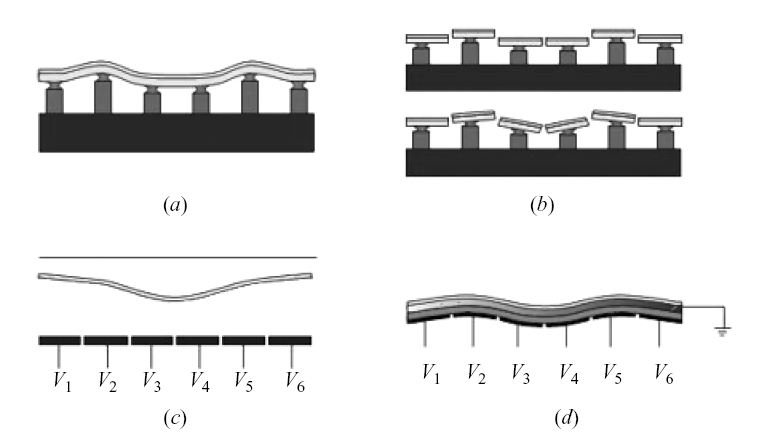
\includegraphics[width=0.45\textwidth]{images/Correctors.png}
	\caption{The four main mirror correctors \cite{AO_vision_science}. (a) Discrete actuator deformable mirrors consist of a continuous, reflective surface and an array of actuators, each capable of producing a local deformation in the surface. (b) Piston-only segmented correctors consist of an array of small planar mirrors whose axial motion (piston) is independently controlled. Piston/tip/tilt-segmented correctors add independent tip and tilt motion to the piston-only correctors. (c) Membrane mirrors and (d) Bimorph mirrors.}
	\label{fig:Correctors}
\end{figure}


Regarding the liquid crystal-based mirrors, they change the refractive index electronically or optically, are wavelength and polarisation dependent and can reach velocities of just a few tens of hertz. The nematic liquid crystal is the most common for AO applications. In general, they are much cheaper than the mirror-based correctors, are capable of producing more complex phase patterns but they have lower light efficiency.   

In AO microscopes the first choice in most cases is the deformable mirror because of their high detection efficiency. Besides, they are better suited for fluorescence techniques due to their polarisation independent behaviour. However, in particular cases, LC-SLM can be enough if aberration correction is only needed in the illumination path.

%%%%%%%%%%%%%%%%%%%%%%%%%%%%%%%%%%%%%%%%%%%%%%%%%%%%%%%%%%%%%%%%%%%%%%%%%%%%%%%
\subsection{Control Strategies}
\label{sec:ControlStrategies}